%************************************************
\chapter{Deep Q-learning with CVaR}\label{ch:dqn}
%************************************************

A big disadvantage of value iteration and Q-learning is the necessity to store a separate value for each state. When the size of the state-space is too large, we are unable to store the action-value representation and the algorithms become intractable. To overcome this issue, it is common to use function approximation together with Q-learning. \citet{mnih2015human} proposed the Deep Q-learning (DQN) algorithm and succesfully trained on multiple different high-dimensional environments, resulting in the first artificial agent that is capable of learning a diverse array of challenging tasks.

In this chapter, we extend CVaR Q-learning to it's deep Q-learning variant and show the practicality and scalability of the proposed methods.

\section{Deep Q-learning}
The ultimate goal of artificial inteligence are agents that perform exhibit a wide range of skills. In the past, research was often focused on narrow AI, which was able to perform well on one particular task, but was unable to generalize to other tasks well. This has changed with the advent of deep learning \citep{krizhevsky2012imagenet}, that allowed us to train function approximators with the ability to generalize. Deep learning methods have become popular across all of machine learning, especially for supervised learning and vision.

\subsection{Deep Learning}

We include a short glossary of deep learning basics and terminology. There are much better sources to draw from and we refer the reader to \citet{goodfellow2016deep} for a comprehensive overview of the field.

Deep learning considers a particular class of parametrized function approximators called \textit{neural networks}. 
Neural networks are functions of the form $f_\theta(x) = f_n \circ f_{n-1} \circ\hdots\circ  f_1(x)$ where $f_i(x) = g_i(\theta_i x)$ with $g_i$ being usually a nonlinear function called the \textit{activation function} and $\theta_i$ is a parameter matrix. Every neural network has an input and output and several \textit{layers}, where a layer represents one matrix multiplication and application of an activation function $f_i(x)$.

The types of neural networks differ, from the simplest with straightforward matrix multiplication called multi layered perceprtons (MLP) to more complicated ones. Arguably the most important layer type that kickstarted the popularity of deep learning is called a \textit{convolutional neural network} or CNN. Convolutional neural network consists of several (even hundreds in recent vision applications) so called convolutional layers and it's input is usually a 2D image. A convolutional layer consists of rectangular filters that look for increasingly abstract features by applying the same weight transformations over the whole image. The takeway from us is that convolutional layers are able to learn from images, which is a fact we utilize in our experiments.

A necessary component of any deep learning algorithm is a loss function $\mathcal{L}$ to be minimized. The most common loss function being the mean squared error
\begin{equation*}
\mathcal{L} = \expval{(f_\theta(x) - \hat{y})^2}
\end{equation*}
with samples $\hat{y}$ representing the outputs drawn from a distribution of interest. 

The loss function is then minimized using Stochastic Gradient Descent, a stochastic version of the well-known gradient descent (see e.g. \citet{boyd2004convex}) where we perform each gradient step only using a subset of available samples. 
%\begin{equation}
%\theta_{t+1} = \theta - \beta\nabla_\theta \mathcal{L}
%\end{equation}
There exist many improved variants of SGD such as RMS-prop \cite{tieleman2012lecture} or Adam \citep{kingma2014adam}, that perform significantly better than the vanilla SGD algorithm and are often used in practice. See \citet{ruder2016overview} for a concise survey of the used algorithms.


\subsection{DQN}

Deep learning has also been succesfully applied to reinforcement learning. Q-learning have been used with function approximators in the past, however it suffers from instabilities during learning. In fact, it is well-known that Q-learning does not converge when used in conjunction with function approximators \citep{baird1995residual, sutton1998reinforcement} and this has been a problem in practice as well. \citet{mnih2015human} were able to stabilize the learning process by introducing two practical techniques. Firstly the model isn't learned online, meaning we see each example once, but instead a replay buffer is used to store transitions $(x, a, r, x')$ and these are later randomly sampled and used repeatedly for the updates. Secondly, a second network $Q'$ is used for computing the target values $r + \gamma Q'(x', a')$ and is only slowly updated towards $Q$. These improvements have helped to stabilize the learning greatly. See \algref{dqn} for the full procedure.

The DQN algorithm has been applied on the Atari Learning Environment \citep{bellemare13arcade}, a set of challenging and diverse tasks, with both inputs and outputs mirroring a human's experience of playing and learning the Atari games, and the same algorithm achieved human and superhuman-level performance on many of these games.

\begin{algorithm}
\caption{Deep Q-learning with experience replay}
\begin{algorithmic}\label{alg:dqn}

    \STATE Initialize replay memory $M$
    \STATE Initialize action-value function $Q$ with random weights $\theta$
    \STATE Initialize target action-value function $Q'$ with weights $\theta'=\theta$

    \FOR{each episode}
    \STATE $x=x_0$
	\WHILE{$x$ is not terminal}
	\STATE Choose $a$ using a policy derived from $Q$ ($\varepsilon$-greedy)
	\STATE Take action $a$, observe $r, x'$
	\STATE Store transition $(x, a, r, x')$ in $M$
	\STATE $x = x'$
	\STATE Sample random transitions $(x_j, a_j, r_j, x_j')$ from $M$
	\STATE Set $\cT Q_j=r_j + \gamma \max_{a'} Q'(x_j', a')$
    \STATE Perform a gradient step on $\bround{\cT Q_j - Q(x_j, a_j)}^2$ w.r.t. $\theta$
    \STATE Every $N_\text{target}$ steps set $\theta'=\theta$
	\ENDWHILE
	\ENDFOR
	
\end{algorithmic}
\end{algorithm}

\section{Distributional Reinforcement Learning with Quantile Regression}\label{sec:dqn:qrdqn}
Before we transition to CVaR Q-learning, we will mention the Quantile Regression DQN algorithm by \citet{dabney2017distributional}, which shares certain similarities with CVaR Q-learning.

In QR-DQN, the goal is to learn a distribution that minimizes the wasserstein distance from the actual return distribution, since the distributional value iteration operator is a contraction in Wasserstein distance. 

The distributions are represented as $N$ discrete uniform atoms with probability $\frac{1}{N}$ and are parametrized with a value that, when learned correctly, represents the $\frac{y_{i}+y_{i+1}}{2}$ quantile, which is the Wasserstein minimizer.

The TD update rule for QR-DQN mimics the quantile estimation introduced in \chref{qlearning}:
\begin{equation*}
V_i(x, a) = V_i(x, a) + \beta \bsquare{1-\dfrac{1}{y_i}\indicator_{(V_i(x, a) \ge \cT V_j)}}
\end{equation*}
where $\cT V_j = r + \gamma V_j(x', a^*)$ and $a^*$ is selected as the action that maximizes the expectated value in the next state. The target is created for each atom $y_j$ separately and differs from the one introduced in CVaR Q-learning.

The loss function reflects the assymetry of the quantile and it is the standart quantile regression loss
\begin{equation}
\sum_{i=1}^{N} \expect_j\bsquare{(\cT V_j - V_i(x, a))(y_j - \indicator_{(V_i(x, a) \ge \cT V_j)})}
\end{equation}
See \figref{losses} for a visual comparison of loss functions used when finding expectations vs quantiles.

\begin{figure}[h]
\center
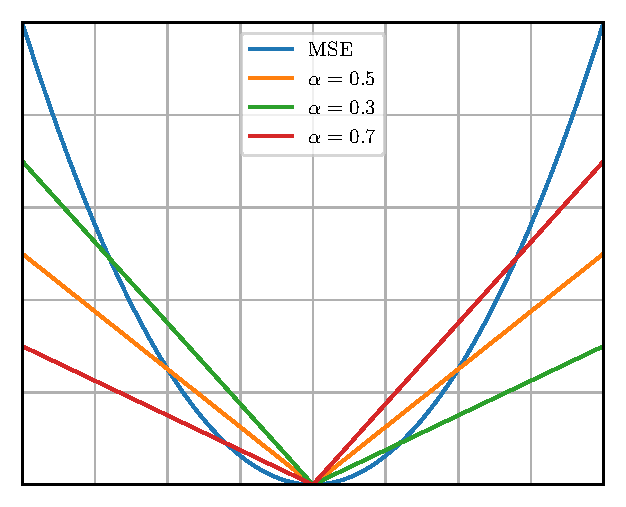
\includegraphics[width=0.6\linewidth]{gfx/losses.pdf}
\caption{Comparison of quantile loss function and Mean Squared Error.}
\label{fig:losses}
\end{figure}

The algorithm is then extended to it's deep Q-learning variant and verified empirically, which is a template we follow in the rest of this chapter.

\section{Deep CVaR Q-learning}
The transition from CVaR Q-learning to Deep CVaR Q-learning (CVaR DQN) follows the same principles as the one from Q-learning to DQN. Recall the TD update rule for CVaR Q-learning:
\begin{align*}
V(x, a, y_i) &= V(x, a, y_i) + \beta \expect_j\bsquare{1 - \dfrac{1}{y_i}\indicator_{(V(x, a, y_i) \ge r+\gamma d_j)}}\\
C(x, a, y_i) &= (1-\beta)C(x, a, y_i) + \beta\expect_j\bsquare{V(x, a, y_i) + \dfrac{1}{y_i}\bround{r+\gamma d_j - V(x, a, y_i)}^-}
\end{align*}
First significant change against DQN or QR-DQN is that we need to represent two separate values - one for $V$, one for $C$. As with DQN, we need to reformulate the updates as arguments minimizing some loss function.

\subsection{Loss functions}
The loss function for $V(x, a, y)$ is similar to QR-DQN loss in that we wish to find quantiles of a particular distribution. The target distribution however is constructed differently - in CVaR-DQN we extract the distribution from the $y\cvar_y$ function of the next state $\cT V = r + \gamma \mathbf{d}$.
\begin{equation}
\mathcal{L}_{\var}=\sum_{i=1}^{N} \expect_j\bsquare{(r + \gamma d_j - V_i(x, a))(y_j - \indicator_{(V_i(x, a) \ge r + \gamma d_j)})}
\end{equation}
where $d_j$ are atoms of the extracted distribution.

Constructing the CVaR loss function consists of transforming the running mean into MSE, again with the transformed distribution atoms $d_j$
\begin{equation}
\mathcal{L}_{\cvar}=\sum_{i=1}^{N} \expect_j\bsquare{\bround{V_i(x, a) + \frac{1}{y_i} \bround{r + \gamma d_j - V_i(x, a)}^- - C_i(x, a)}^2}
\end{equation}


Putting it all together, we are now able to construct the full CVaR-DQN loss function in \algref{cvardqnloss}.

\begin{algorithm}
\caption{Deep CVaR Loss function}
\begin{algorithmic}\label{alg:cvardqnloss}

    \STATE \textbf{input:} $x, a, x', r$
    \bindent
    \FOR{each $y_i$ }
	\STATE $C(x', y_i) = \max_{a'} C(x', a', y_i)$
	\ENDFOR
	
	\STATE $\mathbf{d}= \text{extractDistribution}\bround{C(x', \mathbf{y})}$

	
	\STATE $\mathcal{L}_{\var}=\sum_{i=1}^{N} \expect_j\bsquare{(r + \gamma d_j - V_i(x, a))(y_j - \indicator_{(V_i(x, a) \ge r + \gamma d_j)})}$
	\STATE $\mathcal{L}_{\cvar}=\sum_{i=1}^{N} \expect_j\bsquare{\bround{V_i(x, a) + \frac{1}{y_i} \bround{r + \gamma d_j - V_i(x, a)}^- - C_i(x, a)}^2}$
	\eindent
	\RETURN $\mathcal{L}_{\var} + \mathcal{L}_{\cvar}$
	
\end{algorithmic}
\end{algorithm}

Combining the loss functions with the full DQN algorithm, we get the full CVaR-DQN with experience replay, see \algref{cvardqn}. Note that we also utilize a target network $C'$ that is used for extraction of the target values, similarly to the original DQN. The network $V$ does not have a target network since the target is constructed independently of the value $V$.
\begin{algorithm}
\caption{Deep CVaR Q-learning with experience replay}
\begin{algorithmic}\label{alg:cvardqn}

    \STATE Initialize replay memory $M$
    \STATE Initialize the VaR function $V$ with random weights $\theta_v$
    \STATE Initialize the CVaR function $C$ with random weights $\theta_c$
    \STATE Initialize target CVaR function $C'$ with weights $\theta_c'=\theta_c$

    \FOR{each episode}
    \STATE $x=x_0$
	\WHILE{$x$ is not terminal}
	\STATE Choose $a$ using a policy derived from $C$ ($\varepsilon$-greedy)
	\STATE Take action $a$, observe $r, x'$
	\STATE Store transition $(x, a, r, x')$ in $M$
	\STATE $x = x'$
	\STATE Sample random transitions $(x_j, a_j, r_j, x_j')$ from $M$
	\STATE Build the loss function $\mathcal{L}_{\var} + \mathcal{L}_{\cvar}$ (\algref{cvardqnloss})
    \STATE Perform a gradient step on $\mathcal{L}_{\var} + \mathcal{L}_{\cvar}$ w.r.t. $\theta_v, \theta_c$
    \STATE Every $N_\text{target}$ steps set $\theta_c'=\theta_c$
	\ENDWHILE
	\ENDFOR
	
\end{algorithmic}
\end{algorithm}

%*****************************************
\newpage

\section{Experiments}

To test the approach in a complex setting, we applied the CVaR DQN algorithm to environments with visual state representation, which would be intractable for Q-learning without approximation. 

\subsection{Atari}
We ran several experiments on the Arcade Learning Environment \citep{bellemare13arcade}, which is used as a benchmark for many Deep Q-learning algorithms. The CVaR-DQN algorithm was able to learn reasonable policies with similar speed and performance as the original DQN algorithm. Unfortunately, due to the inherent determinism of the ALE, we didn't find significant differences between policies optimizing $\cvar_\alpha$ on different confidence levels, which led us to the construction of a new visual environment more suitable to risk-sensitive decision making.

\subsection{Ice Lake}
Ice Lake is a visual environment specificaly designed for risk-sensitive decision making. Imagine you are standing on an ice lake and you want to travel fast to a point on the lake. Will you take the a shortcut and risk falling into the cold water or will you be more patient and go around? This is the basic premise of the environment which is visualized in \figref{icelake}.

The agent has five discrete actions, namely go \textit{Left, Right, Up, Down} and \textit{Noop}. These correspond to moving in the respective directions or no operation. Since the agent is on ice, there is a sliding element in the movement - this is mainly done to introduce time dependency and makes the environment a little harder. The enviroment is updated thirty times per second.

The agent recieves a negative reward of -1 per second, 100 if he reaches the goal unharmed and -50 if the ice breaks, then the episode ends. This particular choice of reward leads to about a $10\%$ chance of breaking the ice when taking the shortcut and it is still advantageous for a risk-neutral agent to take the dangerous path.

\begin{figure}[h]
\center
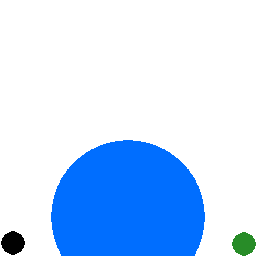
\includegraphics[width=0.3\linewidth]{gfx/icelake_start.png}
\caption{The Ice Lake environment. The agent is black and his target is green. The blue ring represents a dangerous area with risk of breaking the ice. \todo{outline, paths}}
\label{fig:icelake}
\end{figure}

\subsection{Network Architecture}
During our experiments we used the original DQN architecture, including the visual preprocessing trick used in \citet{mnih2015human}.

Firstly, the input images are scaled to $84\times84$ pixels and converted to greyscale to ease memory requirements. In many visual environments, a single image cannot capture the full state information - for example to track the velocity of different objects necessitates to track the objects in time. This problem is solved by concatenating 4 subsequent images which are then used as a single state representation. The input for each state is then of size $84\times84\times4$.

The neural network used in DQN inputs the state representation and outputs a value for each discrete action. The first hidden layer convolves 32 filters of $8\times8$ with stride 4 with the input image and applies a rectifier nonlinearity activation function \citep{jarrett2009best}. The second hidden layer convolves 64 filters of $4\times4$ with stride 2, again followed by a rectifier nonlinearity. This is followed by a third convolutional layer that convolves 64 filters of $3\times3$ with stride 1 followed by a rectifier. The final hidden layer is fully-connected and consists of 512 rectifier units. The output layer is a fully-connected linear layer with a single output for each valid action.
\\
\\
The architecture used in our experiments differs slightly from the original one used in DQN. In our case the output is not a single value but instead a vector of values for each action, representing $\cvar_y$ or $\var_y$ for the different confidence levels $y$. This issue is reconciled by having the output of shape $|\cA|\times N$ where $N$ is the number of atoms we want to use and $|\cA|$ is the action space size.

Another important difference is that we must work with two outputs - one for $C$, one for $V$. We have experimented with two separate networks (one for each value) and also with a single network differing only in the last layer. This approach may be advantageous, since we can imagine that the information required for outputing correct $V$ or $C$ is similar. Furthermore, having a single network instead of two eases the computation requirements.

We tested both approaches and since we didn't find significant performance differences, we settled on the faster version with shared weights. We also used 256 units instead of 512 to ease the computation requirements.

The implementation was done in Python and the neural networks were built using Tensorflow \citep{abadi2016tensorflow} as the framework of choice for gradient descent. The code was based on OpenAi baselines \citep{baselines}, an open-source DQN implementation.

\subsection{Parameter Tuning}
During our experiments, we tested mostly with $\alpha=1$ so as to find reasonable policies quickly. We noticed that the optimal policy with respect to expected value was found fast and other policies were quickly abandoned due to the character of $\epsilon$-greedy exploration. Unlike standart Reinforcement Learning, the CVaR optimization approach requires to find not one but in fact a continuous spectrum of policies - one for each possible $\alpha$. 
This fact, together with the exploration-exploitation dilemma, contributes to the difficulty of learning the correct policies.

After some experimentation, we settled on the following points: 

\begin{itemize}
\item The training requires a higher value of $\epsilon$ than DQN. While in DQN the final $\epsilon$ used during vast majority of the algorithm is 0.01, we settled on $0.3$ as a reasonable value with the ability to explore faster, while making the learned trajectories exploitable.

\item Training with a single policy is insuficcient in larger environments. Instead of maximizing $\cvar$ for $\alpha=1$ as in our CVaR Q-learning experiments, we change the value $\alpha$ for each episode.

\item Because of the way the target is created ***\todo{gradient clipping}
\end{itemize}


\subsection{Results}

With the tweaked parameters, the algorithm was able to converge and learn both the optimal expected value policy and the risk-sensitive policy. See \todo{video or something also atari of something ? moar}

\section{Summary}
We expect that all the DQN improvements such as experience replay \citep{hessel2017rainbow}, dueling \citep{wang2015dueling}, parameter noise \citep{plappert2017parameter} and others (combining the improvements matters, see \citep{hessel2017rainbow}) should have a positive effect on the learning performance, although we stick to vanilla DQN in all of our experiments. huber loss

%*****************************************
%*****************************************
%*****************************************
%*****************************************
%*****************************************
